\chapter{Mapping the room: markers, 3D scan, flight zone, and launching everything}
\label{ch:mapping}
\sloppy

Everything the drone knows about the room is computed \emph{before} the flight, by a handful of offline Python
tools in \file{tools/}, and stored in a few YAML/NPZ files in \file{config/}. During a flight nothing is mapped:
the nodes only \emph{read} these files. This chapter follows the data from the first photo of a marker to the
files the driver loads, then explains how \file{real.launch.py} starts the whole system with them.

The question this chapter answers is the author's own: \emph{``We mapped the room with lots of markers, and did a
3D thing to better draw distances, so we know roughly how far my bed is. We delimited a zone --- how?''} The short
answer is a five-stage pipeline:

\begin{center}
\small
\begin{tabularx}{\textwidth}{@{}l l X >{\raggedright\arraybackslash}p{4.4cm}@{}}
\toprule
Stage & Tool & Input & Output \\
\midrule
1. Marker map & \file{room\_mapper.py} & $\sim$250 Tello photos of the walls, calibration & \file{markers.yaml} (pose of each of the 44 markers in \topic{map}) \\
2. Scan alignment & \file{align\_scan.py} & phone scan (Scaniverse OBJ + texture), marker map & \file{alignment.npz}: similarity $(s, R, t)$ scan $\to$ map \\
3. Scan in \topic{map} & \file{room\_mesh\_to\_map.py} & OBJ + \file{alignment.npz} & \file{room\_map.obj} (+ texture), in metres in \topic{map} \\
4. Flight zone & \file{free\_zone.py} & \file{room\_map.obj}, height band, margin & \file{flight\_zone\_band.yaml}, \file{\_grid.npz}, \file{.png} \\
4'. 3D zone & by hand, viewed with \file{zone\_view.py} & measurements on the scan & \file{flight\_zone\_3d.yaml} (union of 2 boxes) \\
5. Takeoff pad & \file{set\_home.py} & recorded flights & \file{home.yaml} (local, not in git) \\
\bottomrule
\end{tabularx}

\smallskip
Tools are in \file{tools/}, outputs in \file{config/} (except the scan files, kept next to the scan).
\end{center}

\begin{intuition}
The markers give a \emph{precise but sparse} map: 44 small squares on the walls, known to about a centimetre.
The phone scan gives a \emph{dense but floating} model: millions of surface points (walls, wardrobe, desk, bed)
in the phone's own arbitrary frame. The trick is that the markers are \emph{printed on the walls}, so they also
appear in the scan's texture. Finding them there gives point correspondences between the two models, hence the
transform that drops the dense scan into the marker frame. Once the scan is in \topic{map}, ``how far is the
wardrobe'' is just a distance computation on a grid. The flight zone is the set of grid cells, at flight height,
that are at least a margin away from every scanned surface.
\end{intuition}

About the bed: the zone tools only look at surfaces \emph{inside the flight height band} (plus a slack). In band
mode the drone flies between 1.70 and 2.00~m and obstacles are counted between 1.50 and 2.20~m; the bed, the desk
and anything lower than 1.50~m is \emph{deliberately ignored}: the drone flies over it. The scan is what makes the
tall furniture (the wardrobe along the east wall, top at 1.88~m) and the walls visible at that height.

% ======================================================================================================
\section{Stage 1: the marker map (\texorpdfstring{\file{tools/room\_mapper.py}}{room\_mapper.py})}
\label{sec:mapping-mapper}

\subsection{What the tool does}

\file{tools/room\_mapper.py} has three sub-commands:
\begin{lstlisting}
python tools/room_mapper.py calibrate      # 1. camera calibration (checkerboard)
python tools/room_mapper.py capture        # 2. film the markers, drone held by hand, motors off
python tools/room_mapper.py solve          # 3. config/markers.yaml from the saved frames
\end{lstlisting}
No tape measure is needed for the layout: the only metric input is the printed side $\ell$ of the black square.
One image of a marker of known side gives the full 6-DoF pose of that marker relative to the camera; an image
with two markers gives their \emph{relative} pose; chaining these gives a first map; a bundle adjustment then
refines all marker and camera poses together. The final map (Nov~11) was solved from 244 camera poses with a
reprojection RMS of 1.13~px (header of \file{config/markers.yaml}).

\subsection{Module-level helpers}

\func{quat\_xyzw}{(R) -> [x, y, z, w]}
Converts a $3\times3$ rotation matrix to a unit quaternion with Shepperd's method: if the trace
$\operatorname{tr}R > 0$ it uses $w = \tfrac12\sqrt{1+\operatorname{tr}R}$ and
$x = (R_{32}-R_{23})/(4w)$, etc.; otherwise it picks the largest diagonal element as the pivot (the three
\code{elif} branches) to avoid dividing by a small number. The result is renormalised. Used to write the
\code{q} field of every marker.

\func{map\_settings}{() -> (dictionary, marker\_size)}
Reads \code{dictionary} and \code{marker\_size} from the existing \file{config/markers.yaml} (defaults
\code{DICT\_6X6\_50} and 0.15~m if the file is missing). The module constants \code{DICT} and \code{MARKER\_SIZE}
are set from it at import time, so the default \code{--size} of \code{solve} is whatever the current map says
(today 0.1889~m). \code{FLOOR\_CAM\_HEIGHT = 0.035}~m is the camera centre height when the Tello sits on the floor.

\func{aruco\_detector}{() -> callable(gray) -> (corners, ids)}
Builds an OpenCV ArUco detector for \code{DICT} with sub-pixel corner refinement
(\code{CORNER\_REFINE\_SUBPIX}). It supports both the new API (\code{cv2.aruco.ArucoDetector}, OpenCV $\geq$ 4.7)
and the old one (\code{DetectorParameters\_create} + \code{detectMarkers}); both return a lambda with the same
signature.

\func{detect}{(detector, img) -> dict[id -> 4x2 array]}
Grayscale conversion if needed, detection, and conversion to a dictionary \code{\{id: corners\}} with corners in
the OpenCV order top-left, top-right, bottom-right, bottom-left, as \code{float64}. Empty dict if nothing is found.

\func{load\_calib}{(path) -> (K, D, (w, h))} and \func{save\_calib}{(path, K, D, size, rms) -> None}
Read/write the calibration in the ROS \code{camera\_info} YAML layout (\code{camera\_matrix},
\code{distortion\_coefficients} with model \code{plumb\_bob}, identity rectification, projection
$P = [K \mid 0]$), plus the RMS and the date. The file is \file{config/tello\_camera.yaml}.

\func{tello\_stream}{() -> generator of BGR frames}
First checks that the PC is on the Tello Wi-Fi with a trick: \code{connect()} on a UDP socket to
\code{192.168.10.1:8889} sends no packet, but tells which local address the OS would use; if it does not start
with \code{192.168.10.} the program exits with a clear message. Then it connects with \code{djitellopy},
starts the video, skips the black $400\times300$ placeholder frame djitellopy serves before the first decoded
frame, yields each \emph{new} frame (identity test \code{f is not last}) converted RGB$\to$BGR, and in a
\code{finally} block stops the stream and closes the link.

\func{put}{(img, txt, y, color, scale) -> None}
Draws text twice (thick black, then thin coloured) so it is readable on any background.

\subsection{Acquisition: \code{calibrate} and \code{capture}}

\func{cmd\_calibrate}{(a) -> None}
Classic checkerboard calibration: pattern of $9\times6$ inner corners, squares of 25~mm (arguments
\code{--cols}, \code{--rows}, \code{--square}). The 3D model points are the grid $(i\,a, j\,a, 0)$. Each frame
goes through \code{findChessboardCorners}; when found and at least 1~s after the previous view, the corners are
refined with \code{cornerSubPix} (window $11\times11$, 30 iterations or $\varepsilon = 0.001$) and stored. With
$\geq 10$ views, key \textbf{C} runs \code{cv2.calibrateCamera} (pinhole + 5 distortion coefficients, minimising
the reprojection error over all views) and saves with \code{save\_calib}. The on-screen advice is ``25+ views'',
and the RMS is called good below 0.5~px (the current calibration, made with the separate
\file{tools/calibrate\_camera.py}, has 0.24~px).

\func{cmd\_capture}{(a) -> None}
The data acquisition for the map. The operator first puts the drone \emph{on the floor} facing the origin marker
and presses \textbf{F}: the frame is saved as \file{floor\_NN.jpg} (it will give the floor height). Then the drone
is carried by hand along the walls, 1--2~m away, at several heights. Every frame with \emph{at least two}
markers, at most one every \code{--period} = 0.4~s, is saved as \file{f\_NNNNN.jpg} (JPEG quality 95) in
\file{logs/room\_captures/<date>/}. The screen shows how many times each marker was seen and the number of
\emph{linked groups}: two markers are linked if they appeared in the same saved frame; the map can be solved only
if all markers form a single group. Esc stops and prints the command for \code{solve}.

\func{connected\_groups}{(nodes, pairs) -> list of lists}
Union--find (disjoint sets) with path halving (\code{parent[x] = parent[parent[x]]}): each co-visible pair
merges two sets; the groups are the final sets. One group means the co-visibility graph is connected, i.e.\ every
marker can be chained to the origin.

\begin{keypoint}
Why ``2+ markers per frame''? A frame with a single marker gives the camera pose relative to that marker, but
nothing about the \emph{other} markers. Only frames that see several markers carry information about the
relative layout. The co-visibility graph must be connected, otherwise some walls float freely.
\end{keypoint}

\subsection{Geometry helpers for the solve}

Notation: $T_{AB} \in SE(3)$ maps coordinates in frame $B$ to frame $A$:
\[
T_{AB} = \begin{bmatrix} R_{AB} & t_{AB} \\ 0 & 1 \end{bmatrix}, \qquad p_A = R_{AB}\, p_B + t_{AB}.
\]
Frames: $o$ = the origin marker, $c$ = a camera, $i, j$ = markers.

\func{rt\_to\_T}{(rvec, tvec) -> 4x4} / \func{T\_to\_rt}{(T) -> (rvec, tvec)} / \func{inv}{(T) -> 4x4}
Conversions between a Rodrigues rotation vector $r$ (axis $\times$ angle, $R = \exp([r]_\times)$) plus translation
and a homogeneous matrix, and the closed-form inverse
$T^{-1} = \left[\begin{smallmatrix} R^\top & -R^\top t \\ 0 & 1\end{smallmatrix}\right]$.

\func{mean\_rotation}{(Rs) -> R}
The \emph{chordal} mean of rotations: the $R \in SO(3)$ that minimises $\sum_k \lVert R - R_k \rVert_F^2$. Since
$\lVert R - R_k\rVert_F^2 = 6 - 2\operatorname{tr}(R^\top R_k)$, this maximises $\operatorname{tr}(R^\top S)$ with
$S = \sum_k R_k$, whose solution is the projection of $S$ on $SO(3)$: with the SVD $S = U\Sigma V^\top$,
$R = UV^\top$, and if $\det(UV^\top) < 0$ the last column of $U$ is negated to get a proper rotation.

\func{marker\_local}{(size) -> 4x3}
The 4 corners of a marker of side $\ell$ in its own frame (OpenCV convention: $x$ right, $y$ up, $z$ out of the
wall), in detection order:
\[
X^{loc} = \begin{bmatrix} -h & h & 0 \\ h & h & 0 \\ h & -h & 0 \\ -h & -h & 0 \end{bmatrix}, \qquad h = \ell/2 .
\]

\func{single\_pose}{(corners, size, K, D) -> (T\_cam\_marker, err, ratio)}
Pose of one marker from its 4 corners with \code{solvePnPGeneric(..., SOLVEPNP\_IPPE\_SQUARE)}, which returns
\emph{both} solutions of the planar ambiguity (the square tilted one way or the other, see
\file{docs/ARUCO.md}, section 5). The RMS reprojection error of each solution is
taken from OpenCV or recomputed with \code{projectPoints}. It returns the best solution, its error and the
\emph{ambiguity ratio} $\rho = e_2 / e_1$ (second best over best). $\rho \approx 1$ means the two poses explain
the image equally well: do not trust. One solution only: $\rho = 10^9$.

\func{robust\_average}{(Ts, max\_angle\_deg=8) -> (T, n\_kept)}
Fuses several estimates of the same marker pose. First a chordal mean $R_0$ of all rotations, then each estimate
whose rotation is more than $8^\circ$ away is dropped, with the geodesic angle
\[
\theta_k = \arccos\!\left(\frac{\operatorname{tr}(R_0^\top R_k) - 1}{2}\right).
\]
These outliers are the flipped single-marker solutions. If fewer than $\max(1, \lfloor n/3\rfloor)$ survive, all are
kept (no clear consensus). The result is the chordal mean of the kept rotations and the \emph{component-wise
median} of their translations (robust to a few bad positions).

\func{id\_set}{(spec) -> set}
Parses \code{'1-12,15'} into $\lbrace 1,\dots,12,15\rbrace$. Used by \code{--sizes} and \code{--fit-size}.

\func{camera\_from\_known}{(dets, M, size, K, D, single) -> T\_origin\_cam or None}
Locates a camera from the markers of the frame that are already in the map $M$ ($M[i] = T_{oi}$):
\begin{itemize}[nosep]
\item none known: \code{None};
\item one known marker $i$: only if its single-marker pose is trusted, $T_{oc} = T_{oi}\, T_{ci}^{-1}$;
\item several: one joint PnP over all their corners, with 3D points
  $X = R_{oi} X^{loc}_k + t_{oi}$ in the origin frame: \code{SOLVEPNP\_SQPNP} (globally optimal) then
  \code{solvePnPRefineLM}. The pose is accepted only if the RMS reprojection error is below 4~px; it returns
  $T_{oc} = T_{co}^{-1}$.
\end{itemize}

\subsection{\texorpdfstring{\code{cmd\_solve}}{cmd\_solve}: from photos to \texorpdfstring{\file{markers.yaml}}{markers.yaml}}

\func{cmd\_solve}{(a) -> list of marker dicts}
The heart of the tool. It runs in seven steps.

\paragraph{1. Inputs.} The capture folder (\code{--dir}, default the latest one in \file{logs/room\_captures}),
the calibration $K, D$ (or \code{--sim-K f cx cy} with zero distortion, for simulator images), the side of each
marker: \code{--size} for all, overridden per id by \code{--sizes '1-12:0.185;40:0.19'}. Frames are the floor
frames plus every \code{--stride}-th \file{f\_*.jpg}; \code{--floor-from-first N} declares the first $N$ normal
frames to be floor frames instead. Only frames where at least one marker is detected are kept.

\paragraph{2. Trusted single poses and the origin.} For every detection, \code{single\_pose}; it is stored as
trusted only if $e < 1.5$~px \emph{and} $\rho > 3$ (\code{--ambiguity}). The counts and co-visibility (sum of the
number of other markers seen with it) of each marker are accumulated; the origin is \code{--origin} or the marker
with the highest co-visibility (ties: most views). The real map uses marker 49 (130 views, the most of all).

\paragraph{3. Incremental mapping (the ``pairwise'' chaining).} $M = \lbrace o: I_4\rbrace$. Then, up to 50
rounds: for every frame, locate the camera from the known markers (\code{camera\_from\_known}); for every
\emph{new} marker $j$ with a trusted single pose $T_{cj}$ in that frame, propose
\[
T_{oj} = T_{oc}\, T_{cj}.
\]
With a single known marker $i$ this is exactly the pairwise relative pose $T_{ij} = T_{ci}^{-1} T_{cj}$ placed after
$T_{oi}$. A new marker is added when it has at least \code{--min-pairs} = 2 proposals, fused by
\code{robust\_average}. The loop stops when a round adds nothing; markers still missing are reported (``never seen
clearly together with already-mapped markers'') and left out. This is a breadth-first growth of the map over the
co-visibility graph, wall by wall.

\paragraph{4. Initial cameras.} Every frame that can be located from the (now complete) map gets an initial
$T_{oc}$; these frames are the cameras of the bundle adjustment.

\paragraph{5. Bundle adjustment.} The unknown vector stacks, as Rodrigues vector + translation (6 numbers each):
\begin{itemize}[nosep]
\item the pose $T_{oi}$ of every marker \emph{except the origin} (held at the identity);
\item the pose $T_{co}$ of every camera (stored as camera $\leftarrow$ origin, the form \code{projectPoints} wants);
\item optionally one scalar $\log f$, a common size factor for the markers of \code{--fit-size}.
\end{itemize}
With $N_m$ markers and $N_c$ cameras that is $6(N_m - 1) + 6 N_c\ (+1)$ unknowns: for the Nov~11 solve
(42 markers according to its commit, 244 cameras) about $6 \cdot 41 + 6 \cdot 244 = 1710$.
One observation is (camera $c$, marker $i$, its 4 detected corners $u_{cik}$) and gives 8 residuals:
\[
r_{cik} = \pi\!\left(K, D;\ R_{co}\big(R_{oi}\, \sigma_i X^{loc}_k + t_{oi}\big) + t_{co}\right) - u_{cik},
\qquad k = 1..4,
\]
where $\pi$ is the OpenCV pinhole + distortion projection (\code{cv2.projectPoints}), $\sigma_i = e^{x_{-1}}$ for
the markers being size-fitted and 1 otherwise, and $(R_{oi}, t_{oi}) = (I, 0)$ for the origin. The problem
\[
\min_x \ \tfrac12 \sum_{\text{components } m} C^2\, \rho_{\text{Huber}}\!\left(\frac{r_m(x)^2}{C^2}\right),
\qquad \rho_{\text{Huber}}(z) = \begin{cases} z & z \leq 1 \\ 2\sqrt z - 1 & z > 1 \end{cases},
\qquad C = 1\ \text{px}
\]
is solved by \code{scipy.optimize.least\_squares} (trust-region reflective, at most 200 evaluations,
\code{x\_scale='jac'}). The Huber loss is applied by SciPy to each scalar residual: errors above 1~px grow only
linearly, so a badly detected corner cannot dominate. The Jacobian is never formed densely: a boolean
\emph{sparsity pattern} \code{J} (\code{lil\_matrix}) says that the 8 rows of an observation depend only on the 6
columns of its camera, the 6 of its marker (unless origin) and the size factor. SciPy then estimates the Jacobian
by finite differences with column grouping and solves the trust-region steps with the sparse LSMR solver: a few
thousand unknowns are cheap.

\begin{lstlisting}
J = lil_matrix((8 * len(obs), len(x0)), dtype=int)
for k, (ci, i, _) in enumerate(obs):
    J[8 * k: 8 * k + 8, nm + 6 * ci: nm + 6 * ci + 6] = 1       # its camera
    if i != origin:
        J[8 * k: 8 * k + 8, 6 * mi[i]: 6 * mi[i] + 6] = 1       # its marker
    if i in fit:
        J[8 * k: 8 * k + 8, len(x0) - 1] = 1                    # the size factor
\end{lstlisting}

\begin{keypoint}
\textbf{Gauge.} Reprojection errors do not change if \emph{everything} (markers and cameras) is moved by the same
rigid transform: 6 directions of the cost are flat. A monocular problem would also have a free scale (7th
direction). Here the scale is fixed by the known marker sides $\ell$ (the corners $X^{loc}$ are in metres), and
the 6 rigid directions are fixed by holding the origin marker at the identity: it is simply not in the unknown
vector. With \code{--fit-size}, the origin is removed from the fitted set (\code{fit = fit \& set(ids) - \{origin\}})
so the scale stays anchored on the origin's side.
\end{keypoint}

The printed RMS ``before / after'' is $\sqrt{\operatorname{mean}_k \lVert r_k\rVert^2}$ over the corners (the
code multiplies the per-coordinate RMS by $\sqrt2$ for the ``before'' value, the same quantity). If a size factor
was fitted, each fitted side is multiplied by $f = e^{x_{-1}}$ and printed.

\paragraph{6. The \topic{map} frame.} The solution lives in the origin-marker frame, whose axes are those of a
marker on a wall. The \topic{map} frame is built from it:
\begin{itemize}[nosep]
\item \textbf{up}: the mean of the $y$ axes (``up'' on the printed sheet) of all markers,
  $\hat u = \sum_i R_{oi} e_2 / \lVert\cdot\rVert$. Averaging 40+ markers stuck roughly upright gives the
  vertical much better than any single one;
\item \textbf{$y$ axis}: the origin marker's normal $n_0 = R_{oo} e_3$ (out of its wall into the room) made
  horizontal: $y = (n_0 - (n_0 \cdot \hat u)\hat u)/\lVert\cdot\rVert$;
\item \textbf{$x$ axis}: $x = y \times \hat u$, so $(x, y, \hat u)$ is right-handed
  ($x \times y = \hat u$ because $y \perp \hat u$).
\end{itemize}
Stacking them as rows gives the rotation from the origin-marker frame to \topic{map}:
\[
R_{map} = \begin{bmatrix} x^\top \\ y^\top \\ \hat u^\top \end{bmatrix},
\qquad
p^{map} = R_{map}\,(p - p_0) + \begin{bmatrix} 0 \\ 0 \\ z_{off} \end{bmatrix},
\qquad R^{map}_i = R_{map} R_{oi},
\]
with $p_0$ the origin marker's centre. So the map origin is \emph{on the floor right below the centre of
marker 49}, $y$ points into the room, $z$ up: exactly the \topic{map} frame of
\file{docs/ARCHITECTURE.md}. Since the change is a rigid transform applied to everything, it does not change
the reprojection residuals.

The offset $z_{off}$ is the height of the origin marker above the floor, chosen in this order:
\begin{enumerate}[nosep]
\item \code{--origin-height} if given (the real map: 1.95~m, measured with a tape, because floor frames ``taken off
  the floor are misleading'' as the code comment says);
\item otherwise from the floor frames: the median height of those cameras relative to the origin,
  $h_c = \hat u \cdot (t_{oc} - p_0)$ (negative), gives $z_{off} = -(h_c - 0.035)$;
\item otherwise 1.0~m, with a warning.
\end{enumerate}
As a sanity check the median height of the hand-held cameras is printed (1.79~m for the real map).

\paragraph{7. Per-marker report and output.} For each marker: centre in \topic{map}; \code{yaw} $=
\operatorname{atan2}(n_y, n_x)$ of its normal $n = R^{map}_i e_3$ (the direction it faces: $+90^\circ$ for the
south wall, $0^\circ$ for the west wall, $\pm180^\circ$ east, $-90^\circ$ north); \code{tilt} $=
\arccos(R^{map}_{i,(3,2)})$, the angle between its ``up'' axis and the vertical (a marker more than $4^\circ$ off
is flagged ``re-stick it flat and upright''); the number of views; and the median over its observations of the mean
corner residual. With \code{--dry-run} it stops there. Otherwise the old \file{markers.yaml} is backed up as
\file{markers.yaml.bak\_<date>} (several exist in \file{config/}) and a new one is written: header comments
(date, capture, RMS, floor note), \code{dictionary}, \code{marker\_size}, a \code{room} bounding box (marker extent
$+1$~m, height $\max(2.5, z_{max}+0.8)$; used by the simulator only), and one flow-style line per marker
\code{\{id, x, y, z, yaw\_deg, q\}} with an extra \code{size} when it differs from the default. A
\file{solve\_report.json} goes into the capture folder.

\func{main}{() -> None}
Argument parser. The \code{solve} options:

\begin{center}\small
\begin{tabular}{@{}lll@{}}
\toprule
Option & Default & Meaning \\
\midrule
\code{--dir} & latest capture & capture folder \\
\code{--origin} & best connected & origin marker id (real map: 49) \\
\code{--size} & \code{marker\_size} of the map & side of the black square [m] \\
\code{--origin-height} & none & origin marker height [m], overrides floor frames \\
\code{--sizes} & --- & per-id sides, \code{'1-12:0.185;40:0.19'} \\
\code{--fit-size} & --- & ids sharing one unknown size, estimated \\
\code{--stride} & 1 & use one frame out of $N$ \\
\code{--min-pairs} & 2 & proposals needed to place a new marker \\
\code{--ambiguity} & 3.0 & min error ratio to trust a single pose \\
\code{--dry-run} & off & print, do not write \\
\code{--sim-K} & --- & $f, c_x, c_y$ for simulator images \\
\code{--floor-from-first} & 0 & first $N$ frames are floor frames \\
\bottomrule
\end{tabular}
\end{center}
\code{calibrate} takes \code{--cols 9 --rows 6 --square 0.025}; \code{capture} takes \code{--period 0.4}.

\begin{review}
The real map (Nov~11) was solved with \code{--origin-height 1.95} and side 0.1889~m. Two entries of today's
\file{markers.yaml} were \emph{not} produced by this tool: marker 39 (fell on Nov~13, re-located from 4 flight
frames) and marker 18 (``added Nov~16 by hand, NOT measured''). Re-running \code{solve} rewrites the whole file.
\end{review}

% ======================================================================================================
\section{Stage 2--3: the phone scan in the marker frame}
\label{sec:mapping-scan}

The room was scanned with a phone app (Scaniverse, per the docstrings), exported as a textured OBJ: vertices
\code{v}, texture coordinates \code{vt}, triangles \code{f v/vt}, an \file{.mtl} naming a JPEG texture atlas.
The Nov~11 scan used for the current zone (\file{scans/room\_20261111b\_obj/}, outside the repository) has 96\,080
vertices and 170\,142 triangles, no normals. Its frame is the phone's: arbitrary origin, $y$ up (the fitted
rotation maps the scan $y$ axis to the map $z$ axis to within $0.7^\circ$).

\subsection{\texorpdfstring{\file{tools/align\_scan.py}}{align\_scan.py}: finding the similarity}

\func{load\_obj}{(path) -> (V, VT, FV, FT)}
Minimal OBJ reader: $V$ ($n\times3$ positions), $VT$ ($m \times 2$ texture coordinates), and for each triangle the
3 vertex indices $FV$ and the 3 texture indices $FT$ (converted from 1-based to 0-based; only the first 3 corners
of a face are read).

\func{texture\_of}{(obj) -> Path}
The image named by \code{map\_Kd} in the \file{.mtl} next to the OBJ (error if none).

\func{uv\_to\_3d}{(uv, V, VT, FV, FT) -> 3D point or None}
The key idea: a marker corner detected in the \emph{texture image} is a point $p = (u, v)$ of texture space.
Every triangle of the mesh owns a small triangle $(a, b, c)$ of texture space. If $p$ is inside it, with
barycentric coordinates $(w_0, w_1, w_2)$, the same weights applied to the triangle's 3D vertices give the 3D
point where the corner lies on the scanned wall. The barycentric coordinates are computed for all triangles at
once (vectorised) with the standard dot-product formula: with $v_0 = b - a$, $v_1 = c - a$, $v_2 = p - a$ and
$d_{jk} = v_j \cdot v_k$,
\[
w_1 = \frac{d_{11} d_{20} - d_{01} d_{21}}{d_{00} d_{11} - d_{01}^2},\qquad
w_2 = \frac{d_{00} d_{21} - d_{01} d_{20}}{d_{00} d_{11} - d_{01}^2},\qquad
w_0 = 1 - w_1 - w_2,
\]
(the solution of $p - a = w_1 v_0 + w_2 v_1$ in the least-squares sense, exact in 2D). Degenerate triangles
(denominator below $10^{-18}$) get weights $-1$. $p$ is inside when all weights are $\geq -10^{-6}$; the
first such triangle is used:
\[
X = w_0 V_{FV_{k,0}} + w_1 V_{FV_{k,1}} + w_2 V_{FV_{k,2}} .
\]

\func{umeyama}{(src, dst) -> (s, R, t)}
Least-squares similarity between two matched point sets (Umeyama 1991): find $s > 0$, $R \in SO(3)$, $t$
minimising $\sum_k \lVert y_k - (s R x_k + t)\rVert^2$ with $x_k$ = scan points, $y_k$ = map points. The solution:
\[
\mu_x = \tfrac1n\textstyle\sum x_k,\quad \mu_y = \tfrac1n\sum y_k,\quad
\Sigma_{yx} = \tfrac1n \sum (y_k - \mu_y)(x_k - \mu_x)^\top = U S V^\top,
\]
\[
D = \operatorname{diag}\big(1, 1, \operatorname{sign}\det(UV^\top)\big),\qquad
R = U D V^\top,\qquad
s = \frac{\operatorname{tr}(S D)}{\sigma_x^2},\qquad
t = \mu_y - s R \mu_x,
\]
with $\sigma_x^2 = \tfrac1n\sum\lVert x_k - \mu_x\rVert^2$. This is Kabsch's algorithm (centre both sets, SVD of
the cross-covariance, fix a reflection with $D$) plus the optimal scale. Why the scale is unknown: the scan and the
map are two independent metric reconstructions; if they disagree on distances, $s \neq 1$ says so.

\func{main}{() -> None}
\begin{enumerate}[nosep]
\item Loads the marker map (\code{load\_marker\_map}, from \file{src/aruco\_localization}), the OBJ and the
  grayscale texture ($W \times H$).
\item Detects ArUco markers in the \emph{texture image} (same dictionary, sub-pixel corners). Each corner pixel
  $(p_x, p_y)$ becomes the texture coordinate $(p_x/W,\ 1 - p_y/H)$ (OBJ's $v$ axis points up, the image's
  rows down) and then a 3D point with \code{uv\_to\_3d}. A marker counts if it is in the map and all 4 corners
  land on a triangle. Its side in scan units (mean of the 4 edges) is kept for the report.
\item A marker can appear twice in the atlas (the same wall in two charts): its 4 corners are the
  \emph{median} of its instances. At least 3 markers are needed.
\item \textbf{RANSAC} over markers: 300 iterations (fixed seed 0, reproducible); each draws 3 markers (12 point
  pairs), fits \code{umeyama}, and scores every marker by the mean distance of its 4 transformed corners to
  their map positions (\code{corners\_map()}, same corner order). Inliers: mean error below \code{--inlier} =
  6~cm. The best hypothesis has the most inliers, ties broken by the smallest summed error.
\item Final \code{umeyama} on all corners of all inliers.
\item Report per marker: residual, \textbf{leave-one-out} error (refit without that marker, predict it: an honest
  estimate of the alignment error at a place not used for the fit) and side; outliers are flagged ``moved since
  the scan, or wrong in the map?''.
\item Writes \file{alignment.npz} with $s$, $R$, $t$ and the inlier ids (default: next to the OBJ).
\end{enumerate}
For the Nov~11b scan the saved alignment has $s = 0.99992$ and 23 inlier markers.

\begin{intuition}
The scale is how the printer error was found. If the map is solved with an assumed side $\ell'$ while the real
side is $\ell$, every distance of the marker map is multiplied by $\ell'/\ell$, and the alignment of an
(approximately metric) phone scan returns $s \approx \ell'/\ell$. Markers believed to be 20~cm but really 18.89~cm
would give $s \approx 1.059$; the commit of Nov~11 records ``188.9~mm effective marker size from the scan'', and
with the corrected size the scale is now $1.0000$ to $10^{-4}$.
\end{intuition}

\subsection{\texorpdfstring{\file{tools/room\_mesh\_to\_map.py}}{room\_mesh\_to\_map.py}: rewriting the scan in \texorpdfstring{\topic{map}}{map}}

\func{main}{() -> None}
\code{room\_mesh\_to\_map.py <scan.obj> <alignment.npz> <out\_dir> [--ceiling-cut 2.45] [--max-texture 4096]}.
It reads all vertices, keeps the \code{vt} lines and face lines verbatim, and finds the texture in the
\file{.mtl}. Every vertex is transformed (row-vector form of $p^{map} = s R p^{scan} + t$):
\[
M = s\, V R^\top + \mathbf 1 t^\top .
\]
A face is kept only if \emph{all} its vertices are at most \code{--ceiling-cut} = 2.45~m high: the ceiling
disappears, so RViz can look into the room from above. The texture is downscaled (area interpolation) so its
longest side is at most 4096~px (RViz-friendly) and saved as \file{room\_texture.jpg}. It writes
\file{room\_map.obj} (all vertices, transformed; original \code{vt}; kept faces) and \file{room\_map.mtl}
(one unlit material), then prints the counts and the 1st percentile of $z$ (the floor, should be $\approx 0$).
For the Nov~11b scan: 150\,652 of 170\,142 faces kept; vertex heights range from $-0.02$~m (1st percentile) to
2.83~m (99th percentile, the ceiling).

The launch file shows this mesh in RViz if it is copied to \file{\textasciitilde/tello\_ws/room\_scan/room\_map.obj}
(\code{room\_mesh:=auto}, \autoref{sec:mapping-launch}).

% ======================================================================================================
\section{Stage 4: the flight zone (\texorpdfstring{\file{tools/free\_zone.py}}{free\_zone.py})}
\label{sec:mapping-zone}

\subsection{The idea}
At a given height band $[z_{lo}, z_{hi}]$ the room seen from above is a 2D map: a cell is an obstacle if any
scanned surface crosses the band there. The drone's centre must stay at least a margin $m$ away from every
obstacle cell. \file{free\_zone.py} computes, on a 5~cm grid:
\begin{itemize}[nosep]
\item the \textbf{clearance} $c(x, y)$: distance from each cell to the nearest obstacle or to the outside of the
  room (the driver's guard reads it: \file{\_grid.npz});
\item the \textbf{largest free axis-aligned rectangle} (the missions' planning rectangle: the YAML).
\end{itemize}

\subsection{Functions}

\func{load\_obj}{(path) -> (V, F)}
Vertices and the first 3 vertex indices of each face (texture ignored).

\func{surface\_points}{(V, F, step=0.03) -> P}
A mesh vertex every few centimetres is not enough: a large flat face (a wardrobe door) may be 2 big triangles
with vertices only at its corners, and rasterising vertices would leave the door invisible. For every ``big''
triangle ($\max(\lVert b-a\rVert, \lVert c-a\rVert) > 3$~cm) the function adds the points
\[
a + u\,(b - a) + v\,(c - a),\qquad u = \tfrac k6\ (k = 1..5),\quad v = \tfrac j6\ (j = 0..6-k),\quad u+v \leq 1,
\]
i.e.\ 20 interior/edge samples per triangle, on top of all the vertices. For the Nov~11b scan this gives about
979\,000 points.

\func{largest\_rectangle}{(free) -> (i0, i1, j0, j1)}
The classic ``maximal rectangle in a binary matrix'' algorithm, $O(n_x n_y)$. Row by row, $h_j$ is the number of
consecutive free cells ending at the current row in column $j$ (a histogram). The largest rectangle whose bottom
is on this row is the largest rectangle under the histogram, found with a monotonic stack: bars are pushed with
their start column; when a lower bar arrives, the taller ones are popped and each popped bar of height $hh$
started at $s$ gives a candidate area $hh \cdot (j - s)$, rows $[i-hh+1, i+1)$, columns $[s, j)$. A sentinel 0 at
the end flushes the stack. Returns half-open index ranges.

\func{main}{() -> None}
Arguments: \code{obj} (the scan \emph{in the map frame}, from \file{room\_mesh\_to\_map.py}), \code{--z} (default
1.4 2.4), \code{--margin} (0.35), \code{--z-slack} (0.2), \code{--corridor} (0.25), \code{--out}
(\file{config/flight\_zone.yaml}). The steps, with $\Delta = 0.05$~m the cell size:

\begin{enumerate}
\item \textbf{Obstacle points}: $P$ from \code{surface\_points}, kept if
  $z_{lo} - \text{slack} < z < z_{hi} + \text{slack}$. The slack (20~cm) accounts for the height error of the
  drone and the vertical extent of the drone with its cage.
\item \textbf{Grid}: bounds from the 0.5 and 99.5 percentiles of the vertex $x$ and $y$ ($\pm 0.3$~m), so a few
  stray scan points far away do not inflate the grid. Today: $75 \times 99$ cells from $(x_0, y_0) = (-1.56,
  -1.24)$. Each obstacle point marks its cell: $\text{occ}[\lfloor (y - y_0)/\Delta\rfloor, \lfloor (x -
  x_0)/\Delta\rfloor] = 1$ (rows = $y$, columns = $x$; indices clipped to the grid).
\item \textbf{Inside the room}: the scanned walls have holes (windows, doors, missed patches). The occupancy is
  dilated with a $5\times5$ square (2 cells) into \code{walls}, then a flood fill (\code{cv2.floodFill}, 4-connected)
  starts at the cell of the median $(x, y)$ of the floor vertices ($z < 0.1$~m) and marks every non-wall cell it
  reaches. \code{blocked} = \code{occ} $\cup$ \code{$\lnot$inside}.
\item \textbf{Clearance}: Euclidean distance transform of the free cells, in metres,
  \[
  c(p) = \Delta \cdot \min_{q \in \text{blocked}} \lVert p - q\rVert \quad (\text{\code{cv2.distanceTransform}, \code{DIST\_L2}, mask 5}).
  \]
\item \textbf{Margin}: \code{blocked} is dilated with a disc of radius $r = \lceil m/\Delta\rceil$ cells; what
  remains free is where the drone centre may be.
\item \textbf{Mission rectangle}: \code{largest\_rectangle} of the free cells, converted to metres
  $x \in [x_0 + j_0\Delta, x_0 + j_1\Delta]$, $y \in [y_0 + i_0\Delta, y_0 + i_1\Delta]$.
\item \textbf{Main region only}: a morphological \emph{opening} (erosion then dilation) of the free cells with a
  disc of radius $\lceil 0.25/\Delta\rceil = 5$ cells cuts every passage narrower than $\approx 2 \times 0.25$~m;
  \code{connectedComponents} labels the pieces and \code{main} is the one containing the rectangle's centre. The
  alcove in the south-east corner (markers 40 and 41 are at $y = -0.38$ and $-0.65$, behind a narrow gap) is
  thereby excluded. The clearance is then reshaped so that ``$c < m$'' means exactly ``outside \code{main}'':
  \[
  c'(p) = \begin{cases} \min\big(c(p),\ m + d_{in}(p)\big) & p \in \text{main} \\
  \min\big(c(p),\ \max(0, m - d_{out}(p))\big) & p \notin \text{main} \end{cases}
  \]
  with $d_{in}$ the distance to the edge of \code{main} from inside and $d_{out}$ the distance to \code{main} from
  outside. Inside \code{main} the clearance is at least $m$ and grows inwards; outside it falls linearly from $m$
  to 0, which gives the guard a gradient pointing back into the zone.
\item \textbf{Outputs}: \file{<out>\_grid.npz} (\code{clearance}, \code{x0}, \code{y0}, \code{cell}, \code{z\_lo},
  \code{z\_hi}, compressed); the YAML (\code{x\_min \dots z\_max} = rectangle and band, \code{margin},
  \code{grid\_file}); and a PNG top view ($y$ up, $\times 6$): grey = scan vertices, red = obstacles in the band,
  orange = blocked by the margin or outside the main region, green = rectangle.
\end{enumerate}

\subsection{The files the driver uses}
The band zone was made with \code{--z 1.7 2.0 --margin 0.25} (the YAML header records obstacles ``between z 1.50 and
2.20 m'' and margin 0.25; commit of Nov~13: margin $= 0.10$ drone half-size $+ 0.07$ pose error $+$ reserve):
\begin{lstlisting}[language={}]
x_min: -0.86    x_max: 0.94    y_min: 0.36    y_max: 2.76     # 1.80 x 2.40 m
z_min: 1.70     z_max: 2.00    margin: 0.25
grid_file: flight_zone_band_grid.npz
\end{lstlisting}
In the grid, the area with $c' \geq 0.25$~m is 4.56~m$^2$ (the rectangle is 4.32~m$^2$: the driver may use a bit
more than the rectangle), and the largest clearance is 1.20~m (the room centre). The older full-band file
\file{config/flight\_zone.yaml} (1.4--2.4~m, margin 0.35) gives only $1.05 \times 2.20$~m: the taller band meets
more furniture. \autoref{fig:mapping-band} is the PNG of the band zone.

\IfFileExists{../../config/flight_zone_band.png}{%
\begin{figure}[h]
\centering
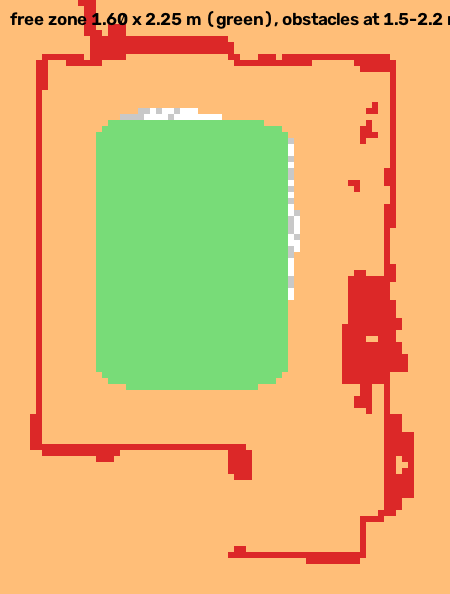
\includegraphics[width=0.42\textwidth]{../../config/flight_zone_band.png}
\caption{\file{config/flight\_zone\_band.png}: top view, $x$ to the right, $y$ up, 5~cm cells. Red: scan surfaces
between 1.50 and 2.20~m (walls; the wardrobe on the east wall). Orange: no-fly (margin, outside, alcove). Green:
the $1.80 \times 2.40$~m mission rectangle.}
\label{fig:mapping-band}
\end{figure}}{}

\paragraph{How they are read.} \file{src/tello\_driver/tello\_driver/zone.py} (\code{load\_zone}) loads the
rectangle, the margin and the grid; \code{make\_grid} adds the gradient $(\partial c/\partial x, \partial
c/\partial y)$ (pointing away from obstacles) and, where the clearance is flat and too small, a vector towards the
nearest cell with room; \code{clearance(zone, x, y)} returns $(c, \text{unit direction})$ at the nearest cell.
The safety layer (\file{safety.py}) brakes and pushes back with it; \file{marker\_map\_publisher} shows the
rectangle (yellow) and the grid as an \code{OccupancyGrid} on \topic{/room/free\_space} (100 where $c < m$).

\subsection{The 3D L-shaped zone (\texorpdfstring{\file{config/flight\_zone\_3d.yaml}}{flight\_zone\_3d.yaml})}

The band is thin (30~cm) because one height must be valid everywhere, and the wardrobe on the east wall
(top at 1.88~m) forbids the east strip at lower heights. The 3D zone (Nov~15) removes that compromise with a
\emph{union of boxes}, where each box is a region the drone \emph{centre} may occupy. It was \textbf{not} computed
by a tool: it was drawn by hand from measurements on the scan, recorded in the file's comments, and checked visually
with \file{tools/zone\_view.py}. Every number can be traced:

\begin{center}\small
\begin{tabular}{@{}llll@{}}
\toprule
Box limit & Value & From (scan / map) & Margin \\
\midrule
west $x_{min}$ & $-0.94$ & west wall $x = -1.24$ & 0.30 \\
\code{main} $x_{max}$ & $0.67$ & furniture front edge $x = 0.92$ & 0.25 \\
upper box $x_{max}$, north part ($y>1.55$) & $1.35$ & east wall $x = 1.65$ & 0.30 \\
upper box $x_{max}$, south part (v1.1) & $1.15$ & high furniture top 1.92~m at $x=1.38$ & 0.27 \\
$y_{min}$ & $0.30$ & south wall $y = 0.0$ & 0.30 \\
$y_{max}$ & $2.87$ & north wall $y = 3.17$ & 0.30 \\
\code{main} $z_{min}$ & $1.55$ & marker row 46/47/39 ($z \approx 1.55$) & --- \\
\code{main} $z_{max}$ & $2.30$ & 0.5~m under the ceiling ($\approx 2.78$) & --- \\
upper box $z_{min}$ & $2.08$ & lowest east marker row 45/34/35/42/43 & --- \\
\bottomrule
\end{tabular}
\end{center}
\begin{lstlisting}[language={}]
margin: 0.25
boxes:
  - {name: main,                 x: [-0.94, 0.67], y: [0.30, 2.87], z: [1.55, 2.30]}
  - {name: above_east_south,     x: [0.67, 1.15],  y: [0.30, 1.55], z: [2.08, 2.30]}
  - {name: above_east_north,     x: [0.67, 1.35],  y: [1.55, 2.87], z: [2.08, 2.30]}
\end{lstlisting}
Seen from the south the union is an ``L'': a tall block over the room and a thin slab over the wardrobe. Its
volume is $1.61 \cdot 2.57 \cdot 0.75 + 0.68 \cdot 2.57 \cdot 0.22 \approx 3.49$~m$^3$ (v1.1, with the south part of the slab trimmed to $x\le 1.15$: $\approx 3.43$~m$^3$), against
$1.80 \cdot 2.40 \cdot 0.30 = 1.30$~m$^3$ for the band zone.

The driver uses it with \code{flight\_zone:=3d}. \code{zone.py} turns it into a clearance grid per height layer
(\code{box\_layers}): the distinct box floors and tops $\lbrace 1.55, 2.08, 2.30\rbrace$ give two layers,
$[1.55, 2.08]$ (only \code{main}) and $[2.08, 2.30]$ (both boxes); for each, on a 2~cm grid, $c = m +
d_{in}$ inside the union and $\max(0, m - d_{out})$ outside, the same shape as $c'$ above. \code{grid\_at}
picks the layer of the current height (5~cm of slack under a layer floor); \code{height\_limits(x, y)} gives the
allowed $[z_{lo}, z_{hi}]$ from the boxes over that point (2.08--2.30~m over the wardrobe).

% ======================================================================================================
\section{Viewing and the takeoff pad}
\label{sec:mapping-view-home}

\subsection{\texorpdfstring{\file{tools/zone\_view.py}}{zone\_view.py}: the 3D HTML viewer}

\func{main}{() -> None}
\code{zone\_view.py <room\_map.obj> [--zone ...3d.yaml] [--markers ...] [--old ...band.yaml] [--voxel 0.03]
[--ceil-cut 2.65] [--out zone\_view.html]}. It builds one self-contained HTML page:
\begin{enumerate}[nosep]
\item the scan surface points (\code{surface\_points} of \file{free\_zone.py}), voxel-downsampled: points are
  keyed by $\lfloor p / 0.03\rfloor$ and \code{np.unique(..., return\_index=True)} keeps the first point of each
  3~cm voxel; coordinates are quantised to centimetres as \code{int16} and base64-encoded (6 bytes per point);
\item the markers (id, position, yaw, quaternion, size) from \file{markers.yaml};
\item the boxes of the 3D zone, its volume, and the band zone as the ``old'' box;
\item the \code{tello\_patrol} default lap: the band rectangle shrunk by 0.35~m, 0.05~m under its top.
\end{enumerate}
The JSON replaces \code{\_\_DATA\_\_} in the page template (\code{PAGE}). In the browser, three.js 0.160.0 (from the
jsDelivr CDN) draws the points coloured by height (blue at 0 to red at 2.4~m), the ceiling points
($z \geq 2.65$, hidden by default), each marker as a black square with its id, the boxes as translucent green
volumes with edges, the band zone as a yellow wireframe (the RViz colour) and the patrol path in orange, with
\code{OrbitControls} ($z$ up) and checkboxes to toggle each layer. The interface text is in French.

\subsection{\texorpdfstring{\file{tools/set\_home.py}}{set\_home.py}: the takeoff pad}

The drone always takes off from marker 48 lying on the floor (not in the map). Its camera looks forward and never
sees the pad, but the drone climbs straight up after takeoff, so the first wall-marker poses of each climb give the
takeoff point. \file{config/home.yaml} is local (in \file{.gitignore}); the EKF starts there before any marker is
seen, and the missions land on it.

\func{rows}{(path) -> list of dicts}
A CSV file as dictionaries (empty list if missing).

\func{takeoff\_point}{(ses) -> (x, y, yaw\_deg, n) or None}
From a session folder: $t_{up}$ = first telemetry row with \code{flying == True}; the ArUco poses
(\file{poses.csv}) in $(t_{up}, t_{up} + 8\,\text{s})$ (takeoff and climb, before any horizontal move; at least 3);
then the poses of the \emph{first second} of that window. Position = median $x$, median $y$; heading = circular
median-like average $\operatorname{atan2}(\operatorname{median}\sin\psi, \operatorname{median}\cos\psi)$ (correct
across $\pm180^\circ$).

\func{landing\_point}{(ses) -> (x, y) or None}
Median pose between 4 and 2~s before the last \code{flying} sample (just before the descent). Not used by
\code{main}; \file{tools/flight\_report.py} imports it to check the landing on the pad.

\func{load}{() -> dict}
The current \file{home.yaml} or \code{\{\}}.

\func{main}{() -> None}
Without arguments it adds the latest session of \file{\textasciitilde/tello\_ws/sessions/}; with paths, those;
\code{--reset} forgets the history (writes only \code{pad\_marker}). Sessions already in the history are skipped.
Each new takeoff is appended as \code{[x, y, yaw, session]}. The pad is then estimated robustly:
\[
(\tilde x, \tilde y) = \operatorname{median}, \quad
\text{keep} = \lbrace k : \lVert (x_k, y_k) - (\tilde x, \tilde y)\rVert < 0.25\,\text{m}\rbrace, \quad
(x, y) = \operatorname{median}_{\text{keep}},
\]
the heading by the same circular formula, and the spread (std of the distances) is printed. It writes \code{pad\_marker},
\code{x}, \code{y}, \code{yaw\_deg}, \code{samples} and the full \code{history}, and lists the flights rejected as
``not from the pad''.

% ======================================================================================================
\section{Launching everything}
\label{sec:mapping-launch}

\subsection{\texorpdfstring{\file{src/tello\_driver/launch/real.launch.py}}{real.launch.py}}

\code{REPO} is \code{\$TELLO\_REPO} or \file{\textasciitilde/tello\_ws/src/tello-balloon-hunter}: all config files are
read from the repository (inside WSL), not from the install space, so editing a YAML needs no rebuild.

\paragraph{\code{LOCAL\_ROS\_ENV}.} Three environment variables are set for every node
(\code{SetEnvironmentVariable}): \code{ROS\_AUTOMATIC\_DISCOVERY\_RANGE=LOCALHOST} (discovery only on this machine),
\code{FASTDDS\_BUILTIN\_TRANSPORTS=LARGE\_DATA}, and \code{FASTRTPS\_DEFAULT\_PROFILES\_FILE} pointing to the installed
\file{fastdds\_local.xml} (below). Reason (comment of Nov~10): Windows switches to the Tello Wi-Fi (no multicast,
no internet), WSL mirrored networking drops fragmented UDP on the loopback, and with Tailscale running the discovery
packets grew beyond 1500 bytes; the nodes stopped seeing each other.

\func{setup}{(context) -> list of Node}
The \code{OpaqueFunction} body, run when the arguments are known. It first runs \code{fastdds shm clean} (timeout
15~s, errors ignored): shared-memory segments left by killed ROS processes could silently block RViz. Then it
resolves the zone, takeoff height and calibration and returns the nodes:

\begin{center}\small
\begin{tabularx}{\textwidth}{@{}l X@{}}
\toprule
Node (package / executable) & Parameters \\
\midrule
\code{tello\_driver/tello\_driver} & \code{mock} (bool), \code{camera\_info\_file}, \code{mock\_markers\_file} = markers,
  \code{takeoff\_height} = climb, \code{max\_height}, \code{flight\_zone\_file} = zone \\
\code{aruco\_localization/marker\_map\_publisher} & \code{markers\_file}, \code{room\_mesh}, \code{flight\_zone\_file} \\
\code{tello\_driver/tello\_ekf} & none (defaults; reads \file{home.yaml} itself) \\
\code{aruco\_localization/aruco\_localizer} & \code{markers\_file}, \code{child\_frame = base\_link\_aruco} (the EKF owns
  \topic{base\_link}), \code{debug\_every\_n = 3}, \code{debug\_scale = 0.5} \\
\code{tello\_driver/session\_recorder} & if \code{record:=true} \\
\code{rviz2} & if \code{rviz:=true}; \code{-d} a copy of \file{real.rviz} centred on the markers; output to log \\
\bottomrule
\end{tabularx}
\end{center}
With \code{mock:=true} the same nodes run, but the driver instantiates \code{FakeTello} (\file{fake\_tello.py}) with
the marker map as its virtual world, so the localizer, EKF and RViz are exercised without hardware.

\func{zone\_file}{(arg, band=False) -> path or ""}
\code{none} $\to$ no zone; \code{3d} $\to$ \file{config/flight\_zone\_3d.yaml}; any other value except \code{auto} is
used as a path; \code{auto} $\to$ \file{flight\_zone\_band.yaml} in band mode, else \file{flight\_zone.yaml}, if it
exists.

\func{room\_mesh}{(arg) -> path or ""}
\code{auto} $\to$ \file{\textasciitilde/tello\_ws/room\_scan/room\_map.obj} if it exists.

\func{takeoff\_height}{(markers\_file, arg, band\_zone="") -> float}
A number is used as is. With \code{auto} in band mode: the middle of the zone's height range (band file:
$(1.70+2.00)/2 = 1.85$~m; 3D file: the min floor and max top of the boxes, $(1.55+2.30)/2 \to 1.92$~m). Otherwise
from the markers: median marker height $- 0.3$~m, clipped to $[1.0, 2.0]$ (today $2.224 - 0.3 = 1.92$~m); 0.0
if the map cannot be read.

\func{rviz\_config\_centred\_on\_markers}{(template, markers\_file) -> path}
Rewrites four lines of \file{real.rviz} by plain string replacement: the orbit focal point becomes the markers'
centroid; the distance $\max(4, 1.6 \cdot \text{span})$; the grid offset the centroid rounded to 0.5~m (lines on
round coordinates); the view yaw the direction of the mean marker normal $\operatorname{atan2}(\sum\sin\psi_i,
\sum\cos\psi_i)$, so the printed faces are visible. Written to \file{/tmp/tello\_real\_centred.rviz}; on any error
the template is used unchanged.

\func{generate\_launch\_description}{() -> LaunchDescription}
The environment variables, the arguments, and the \code{OpaqueFunction(setup)}:

\begin{center}\small
\begin{tabularx}{\textwidth}{@{}l l X@{}}
\toprule
Argument & Default & Meaning \\
\midrule
\code{mock} & false & fake drone \\
\code{rviz} & true & start RViz \\
\code{record} & true & \code{session\_recorder} into \file{\textasciitilde/tello\_ws/sessions} \\
\code{markers} & \file{REPO/config/markers.yaml} & marker map \\
\code{band} & true & band mode: zone \file{flight\_zone\_band.yaml}, climb to its middle \\
\code{flight\_zone} & auto & \code{auto} / \code{3d} / \code{none} / a path \\
\code{room\_mesh} & auto & scan OBJ in \topic{map} \\
\code{max\_height} & 2.6 & ceiling guard [m] \\
\code{takeoff\_height} & auto & climb after takeoff [m]; 0 = none \\
\code{camera\_info\_file} & auto & \file{REPO/config/tello\_camera.yaml} if present \\
\bottomrule
\end{tabularx}
\end{center}

\subsection{Entry points (\texorpdfstring{\file{src/tello\_driver/setup.py}}{setup.py})}
\code{setup.py} installs the package, the launch files and every file of \file{config/} (\file{real.rviz},
\file{fastdds\_local.xml}) into the share directory, and declares ten console scripts, i.e.\ the
\code{ros2 run tello\_driver <name>} commands:

\begin{center}\small
\begin{tabular}{@{}ll@{}}
\toprule
\code{ros2 run tello\_driver \dots} & Module \\
\midrule
\code{tello\_driver} & \code{driver:main} \\
\code{tello\_teleop} & \code{teleop:main} \\
\code{tello\_step\_test} / \code{tello\_step\_fit} & \code{step\_test:main} / \code{step\_fit:main} \\
\code{tello\_marker\_tour} & \code{marker\_tour:main} \\
\code{tello\_goto} & \code{goto\_markers:main} (e.g.\ \code{tello\_goto 49 35}) \\
\code{tello\_ekf} & \code{ekf\_node:main} \\
\code{tello\_strike} & \code{strike:main} \\
\code{tello\_patrol} & \code{patrol:main} \\
\code{session\_recorder} & \code{session\_recorder:main} \\
\bottomrule
\end{tabular}
\end{center}

\subsection{\texorpdfstring{\file{tello.bat}}{tello.bat} and \texorpdfstring{\file{scripts/wsl/}}{scripts/wsl}}

\textbf{\file{tello.bat}} (double-click on Windows; \code{tello.bat mock} for the fake drone):
\begin{enumerate}[nosep]
\item Wi-Fi (skipped for \code{mock}): connects the USB dongle interface \code{Wi-Fi 2} to SSID
  \code{TELLO-5F897A} with \code{netsh wlan connect}, checking \code{netsh wlan show interfaces} every 3~s, at most 20
  tries (60~s), then a troubleshooting message. The built-in card stays on the internet.
\item ROS: a new window runs, in WSL, \code{source /opt/ros/jazzy/setup.bash}, the workspace, \file{ros\_env.sh},
  then \code{ros2 launch tello\_driver real.launch.py [mock:=true]}; the window title reminds that Ctrl+C there lands
  and stops everything.
\item After 8~s, a second WSL window with the same environment, in the repository, printing the usual commands
  (teleop, \code{tello\_goto 49 35}, \code{flight\_report.py --band 1.7 2.0}).
\end{enumerate}

\textbf{\file{scripts/wsl/ros\_env.sh}} exports the same three variables as \code{LOCAL\_ROS\_ENV}, so that command-line
tools (\code{ros2 topic echo} \dots) in another terminal join the same local-only DDS domain as the launched
nodes.

\textbf{\file{scripts/wsl/setup\_ros\_jazzy.sh}} prepares Ubuntu 24.04 (checks \code{noble}) in six idempotent steps:
(1) the ROS 2 apt source (\code{ros2-apt-source} .deb, latest release from GitHub); (2) \code{ros-jazzy-desktop},
\code{ros-dev-tools}, cv\_bridge, camera calibration, teleop, usb\_cam, OpenCV, PIL, YAML, pip, git; (3)
\code{djitellopy} and PyAV with \code{pip --user --no-deps} (a pip numpy~2 would break the system OpenCV /
cv\_bridge); (4) clone or \code{pull --ff-only} the repository into \file{\textasciitilde/tello\_ws/src} (on the Linux
disk, not OneDrive); (5) \code{colcon build --symlink-install} of \code{aruco\_localization} and \code{tello\_driver};
(6) source lines in \file{\textasciitilde/.bashrc}, then an import check.

\subsection{\texorpdfstring{\file{fastdds\_local.xml}}{fastdds\_local.xml}}
A Fast DDS profile made the default for every participant (\code{is\_default\_profile="true"}):
\begin{itemize}[nosep]
\item two user transports: \textbf{SHM} (shared memory, segment 16~MiB: a $960\times720$ BGR image is 2~MB) and
  \textbf{UDPv4 restricted to 127.0.0.1} with \code{maxMessageSize} 1400 bytes (no IP fragmentation, which WSL
  drops on the loopback);
\item \code{useBuiltinTransports=false}: the default transports (UDP on every interface) are not created;
\item metatraffic (discovery) unicast locator and initial peer: 127.0.0.1.
\end{itemize}
The effect: discovery and data never leave the PC, whatever Wi-Fi Windows is on.

\subsection{\texorpdfstring{\file{real.rviz}}{real.rviz}: the displays}
Fixed frame \topic{map}, 30~fps, an orbit view (rewritten by the launch file), and the tools Interact, MoveCamera,
Select, FocusCamera, Measure (the Measure tool gives distances in the scene: a quick way to read ``how far is
the wardrobe'' on the scan).

\begin{center}\small
\begin{tabularx}{\textwidth}{@{}l l X@{}}
\toprule
Display & Topic & What it shows \\
\midrule
Grid & --- & 0.5~m cells, 10 per side, in \topic{map}, offset under the room \\
TF & --- & all frames with names (\topic{map}, \topic{aruco\_<id>}, \topic{base\_link}, \topic{base\_link\_aruco}, camera) \\
Room (3D scan) & \topic{/room/mesh} & the textured \file{room\_map.obj} (Marker \code{MESH\_RESOURCE}, transient local) \\
Free space & \topic{/room/free\_space} & \code{OccupancyGrid}: black = no-fly ($c < m$), alpha 0.35 \\
Flight zone & \topic{/room/flight\_zone} & yellow = band zone the driver enforces; green = boxes of the 3D zone \\
ArUco markers & \topic{/aruco/map\_markers} & each marker as a white sheet + black square + id \\
Drone & \topic{/tello/body\_markers} & body, propellers, heading arrow, camera field of view \\
Markers seen now & \topic{/aruco/sight\_lines} & green lines camera $\to$ markers used in the current pose \\
Drone trajectory & \topic{/ekf/path} & EKF path, orange \\
ArUco pose (raw) & \topic{/aruco/pose} & axes of the raw marker pose (disabled by default) \\
Tello camera & \topic{/aruco/debug\_image} & image with detections and OK / REJECTED \\
\bottomrule
\end{tabularx}
\end{center}
With \code{flight\_zone:=3d} the YAML has no \code{grid\_file}, so the Free space display stays empty and only the
green boxes are drawn (the publisher checks for the key \code{boxes}).

% ======================================================================================================
\section{Summary: from the room to the YAML files}

\begin{enumerate}[nosep]
\item Calibrate the Tello camera ($K$, distortion; 0.24~px).
\item Carry the drone along the walls; 244 frames with $\geq 2$ markers; the co-visibility graph must be connected.
\item Single-marker poses (IPPE, trusted if $e < 1.5$~px and $\rho > 3$) $\to$ incremental chaining from marker 49
  $\to$ bundle adjustment over all corners (Huber, sparse, origin fixed, scale from $\ell = 0.1889$~m) $\to$ map
  frame (vertical = mean marker ``up'', $y$ = normal of 49, origin on the floor 1.95~m below 49) $\to$
  \file{markers.yaml}.
\item Scan the room with the phone; detect the markers in the texture; lift the corners to 3D by barycentric
  interpolation; RANSAC + Umeyama similarity ($s = 0.9999$, 23 markers) $\to$ \file{alignment.npz} $\to$
  \file{room\_map.obj} in \topic{map}.
\item Slice the scan at 1.50--2.20~m, rasterise at 5~cm, flood-fill the inside, distance transform, 0.25~m margin,
  largest rectangle, main region $\to$ \file{flight\_zone\_band.yaml} + grid; hand-drawn L zone from the same scan
  $\to$ \file{flight\_zone\_3d.yaml}.
\item Fly from the pad; \file{set\_home.py} $\to$ \file{home.yaml}.
\item \code{tello.bat} $\to$ \code{real.launch.py} reads all of them.
\end{enumerate}

% ======================================================================================================
\section{Code review notes}

All points below were checked in the code (and, where stated, against the data in \file{config/} and the scan in
\file{../scans/room\_20261111b\_obj/}). No code was modified.

\begin{review}
\begin{enumerate}[leftmargin=*]
\item \textcolor{OliveGreen}{\textbf{[Fixed in v1.1, see Appendix~\ref{app:review}.]}} \textbf{\file{config/flight\_zone\_3d.yaml}:10 --- the stated check does not hold.} The comment says ``no scan
  point inside a box grown by 0.25 m''. Re-running the test with \code{surface\_points} on
  \file{room\_map.obj}: 3105 points fall in the \code{above\_east\_furniture} box grown by 0.25~m, and points up to
  $z = 1.90$~m lie \emph{directly under} that box ($x \approx 1.33$--$1.35$, $y$ 0.55--1.38), i.e.\ only 0.18~m
  below its 2.08~m floor. The test passes with a growth of 0.15~m, not 0.25~m. Since \file{safety.py}:247 tolerates
  0.10~m below the floor of the allowed height range before reacting, the cage could come within $\sim$8~cm (centre)
  of the wardrobe top. Raise that box floor to $\approx 2.15$~m or trim its east edge.
\item \textcolor{OliveGreen}{\textbf{[Fixed in v1.1, see Appendix~\ref{app:review}.]}} \textbf{\file{config/flight\_zone\_3d.yaml}:1--2 --- stale status.} ``Not used by the driver yet'', but
  \file{real.launch.py}:73 accepts \code{flight\_zone:=3d} and \file{zone.py}:70 enforces it (layers, height
  limits). The reader may believe the zone is only decorative.
\item \textbf{\file{tools/free\_zone.py}:91--100 --- hidden extra margin.} The $5\times5$ dilation meant to close
  holes before the flood fill also defines \code{inside}, so every obstacle is effectively grown by 2 cells
  (0.10--0.14~m) before the distance transform. The clearance in \file{\_grid.npz} is therefore measured to the grown
  obstacles: the real margin is $\approx m + 0.1$~m, not the $m$ written in the YAML. Safe, but undocumented;
  dilating the flooded region back by the same 2 cells would restore the exact margin.
\item \textbf{\file{tools/free\_zone.py}:94--98, 120 --- unchecked seeds.} The flood-fill seed (median of the
  floor vertices) is not clipped nor tested: if it falls on a dilated obstacle, \code{floodFill} fills the
  \emph{walls} instead of the room; out of range, it raises. Likewise \code{lab[...]} at the rectangle centre may be
  the background label 0 after the opening, making \code{main} the whole non-free area. Assert
  \code{ff[seed] == 1} and \code{label != 0}.
\item \textbf{\file{tools/free\_zone.py}:4,71--72 --- docstring defaults wrong.} The usage line says
  \code{--z 1.2 2.4 --margin 0.5}; the code defaults are 1.4 2.4 and 0.35 (and the band file uses 1.7 2.0, 0.25).
  Also :146 draws a caption wider than the image: it is cut in \file{flight\_zone\_band.png}.
\item \textbf{\file{tools/set\_home.py}:252--255 --- NaN pad.} If no sample lies within 0.25~m of the
  coordinate-wise median (e.g.\ two flights more than 0.5~m apart), \code{keep} is all \code{False}, the medians of
  empty arrays are NaN and \code{x: nan} is written to \file{home.yaml}; \file{home.py} \code{load\_home} parses it
  with \code{float()} and the EKF would be initialised at NaN. Fall back to all samples when \code{keep.sum() == 0}.
\item \textbf{\file{tools/room\_mapper.py}:483 --- vertical from all markers.} ``Up'' is the mean $y$ axis of
  \emph{every} mapped marker. A marker on the floor or ceiling (e.g.\ the pad marker 48 if it ever appears in a
  capture) has a horizontal $y$ axis and would tilt the whole map. Exclude markers whose $y$ axis is far from the
  mean (the tilt test already exists at :512).
\item \textbf{\file{tools/room\_mapper.py}:528--553 --- hand edits lost on re-solve.} The file is rewritten from the
  solve only: marker 18 (hand-placed, not measured) would disappear and marker 39's re-location note would be
  overwritten. Backups exist, but nothing warns. Also stale texts: :8 says markers are 15~cm (0.1889 today),
  :351 mentions a ``menu choice 7'' that does not exist, :33 adds \file{scripts/} to \code{sys.path} for nothing,
  and \file{config/markers.yaml}:2 says \file{scripts/room\_mapper.py}.
\item \textbf{\file{tools/room\_mesh\_to\_map.py}:43, 62--64 --- face lines copied verbatim.} Only \code{v} and
  \code{vt} lines are written; a scan exported \emph{with} normals (\code{f v/vt/vn}) would reference missing
  \code{vn} lines (and normals would not be rotated). The current Scaniverse export has no \code{vn} (checked), so it
  works today. Line 39 also fails if there is no \file{.mtl}.
\item \textbf{\file{src/tello\_driver/launch/real.launch.py}:90 --- docstring vs code.} The docstring says ``0.5 m
  under the median marker height''; the code (:110) uses 0.3~m (on purpose, comment at :108).
\item \textbf{\file{scripts/wsl/setup\_ros\_jazzy.sh}:145--150 --- \file{ros\_env.sh} never sourced.}
  \file{ros\_env.sh}:1--2 says to source it in \file{\textasciitilde/.bashrc}, but the setup script only adds the ROS
  and workspace setup files. A plain WSL terminal then uses default discovery and may not see the launched nodes
  (the \file{tello.bat} windows do source it).
\item \textbf{\file{tools/zone\_view.py}:7 --- minor.} The docstring says the band zone is a ``grey wireframe''; it
  is drawn yellow (:93). Files are opened without \code{encoding} (:126--130), which on Windows means cp1252; the
  YAMLs are ASCII today.
\end{enumerate}
\end{review}
ussy
